\documentclass{article}
%\usepackage[spanish,activeacute]{babel}
%\usepackage[english,activeacute]{babel}
%\usepackage[latin1]{inputenc}
\usepackage[utf8]{inputenc}
\usepackage[english]{babel}

\usepackage{amsmath,amsfonts,amssymb,amstext,amsthm,amscd}
\usepackage{hyperref}
\usepackage{latexsym}
\usepackage{graphicx}
%\usepackage{subfigure}
\usepackage{subfig}
%\linespread{1.6}
\usepackage{float}
\usepackage{dcolumn}% Align table columns on decimal point(esto lo saque del ejemplo de revtex4)
\usepackage{bm}% bold math(esto lo saque del ejemplo de revtex4)
\newcounter{itemR}
\usepackage{here} %recordar usar el comando[H] para las gráficas que es el comando here en lugar de [h!]
\usepackage{fancyhdr}
%\usepackage{sidecap}
%\usepackage[spanish,activeacute]{babel}
\usepackage{multirow}
\usepackage{multicol}
\usepackage{array}
\usepackage{enumitem}
%\usepackage{booktabs}% para hacer tablas profesionales con \toprule

% ------------------------------------------------------------------------------------------------------------------------------------------------------

\usepackage{fancyhdr}
\setlength{\headheight}{15.2pt}
\usepackage[paperwidth=8.5in, paperheight=11.0in, top=1.0in, bottom=1.0in, left=1.0in, right=1.0in]{geometry}

\pagestyle{fancyplain}
\fancyhead[LE,RO]{Práctica $\#$1 \& 2, Faraday, fuerza electrica}
\fancyhead[CE,CO]{}
\fancyhead[RE,LO]{P23-FIS1012-12}
\fancyfoot[LE,RO]{\thepage}
\fancyfoot[CE,CO]{Laboratorio de Física, UDLAP}
\fancyfoot[RE,LO]{}

% ------------------------------------------------------------------------------------------------------------------------------------------------------
% ------------------------------------------------------------------------------------------------------------------------------------------------------
% ------------------------------------------------------------------------------------------------------------------------------------------------------

\begin{document}

\fancypagestyle{plain}{
   	\renewcommand{\headrulewidth}{1pt}
   	\renewcommand{\footrulewidth}{1pt}
}

\renewcommand{\footrulewidth}{1pt}
\renewcommand{\tablename}{Tabla}
\renewcommand{\figurename}{Figura}

% ------------------------------------------------------------------------------------------------------------------------------------------------------
% ------------------------------------------------------------------------------------------------------------------------------------------------------
% ------------------------------------------------------------------------------------------------------------------------------------------------------

\title{Carga y fuerza eléctrica}
\author{\small{Luis Alberto Gil Bocanegra ID: 177410, Erick Gonzalez Parada ID: 178145}\\
 \small{Gartzen Aldecoa Barroso ID: 178034 .}\\		% ----- Varios autores separarlos por comas:  \small{Nombre(s) de (los) autor(es)\footnote{ID; correo@udlap.mx}, Nombre(s) de (los) autor(es)\footnote{ID; correo@udlap.mx}
	   \small{Depto. de Actuaría, Física y Matemáticas, Universidad de las Américas Puebla, Puebla, M\'exico 72810}}
\date{\small{\today}}

\maketitle

% ------------------------------------------------------------------------------------------------------------------------------------------------------
% ------------------------------------------------------------------------------------------------------------------------------------------------------
% ------------------------------------------------------------------------------------------------------------------------------------------------------

\begin{abstract}
	Durante las 3 prácticas se observo los tipos de carga de maneras diferentes 
	con diferentes estrategias como frotar objetos o generando electricidad directamente 
	con ayuda de generadores de electrones como la máquina de Wimshurst. 
\\
\\
{\it Keywords:}  campo, electricidad, lineas equipotenciales  
\\
\\
\end{abstract}

% ------------------------------------------------------------------------------------------------------------------------------------------------------

\begin{multicols}{2}

\section{Desarrollo teórico}\label{Desarrollo Teorico}                              	% -------------------- Introducción
\subsection{Objetivo primera práctica}\label{Objetivo primera práctica}
	Observar la existencia y tipos de carga
	\subsection{marco teórico \ref{Objetivo primera práctica}}
	\paragraph*{Carga eléctrica}
	La carga eléctrica es una propiedad fundamental de la materia que se manifiesta debido 
	a la interacción de partículas subatómicas, como electrones (\ensuremath{-e^{-}}) y protones 
	(\ensuremath{+p^{+}}). Los electrones tienen una carga eléctrica negativa
	(\ensuremath{q_{e}=-1.602\times 10^{-19}\mathrm{C}}), mientras que los protones
	tienen una carga eléctrica positiva (\ensuremath{q_{p}=1.602\times 10^{-19}\mathrm{C}}).
	La carga eléctrica es una propiedad cuantizada, lo que significa que solo puede existir 
	en múltiplos enteros de la carga elemental.

	\paragraph*{Tipos de carga eléctrica}
	\cite{Serway}
\begin{enumerate}
\item Carga Positiva: Producida por protones (\ensuremath{+p^{+}}), tiene una polaridad positiva (\ensuremath{q>0}).
\item Carga Negativa: Producida por electrones (\ensuremath{-e^{-}}), tiene una polaridad negativa (\ensuremath{q<0}).
\item Carga Neutra: Un objeto es eléctricamente neutro cuando tiene un número igual de protones y electrones, lo que resulta en una carga neta de cero (\ensuremath{q=0}).
\item Carga Ionizada: Un átomo o molécula puede ganar (\ensuremath{q>0}) o perder (\ensuremath{q<0}) electrones, formando iones con carga eléctrica.
\item Carga Cuantizada: La carga eléctrica viene en múltiplos de la carga elemental (\ensuremath{q_{e}=1.602\times 10^{-19}~\mathrm{C}}).
\end{enumerate}

\subsection{Objetivo segunda práctica}\label{Objetivo segunda práctica}	
	Determinar la carga, observar los dos tipos de carga, inducción y depósito de carga.
	\subsection{marco teórico \ref{Objetivo segunda práctica}}
	\paragraph*{inducción y depósito de carga}
	La inducción eléctrica se refiere al proceso mediante el cual se redistribuyen
	las cargas eléctricas en un objeto debido a la influencia de un campo eléctrico externo,
	sin que haya contacto físico directo con otro objeto cargado. A continuación, se describen
	los conceptos clave:

	\begin{enumerate}
		\item Carga Inducida: Cuando un objeto cargado se acerca a un objeto neutro, el campo eléctrico del primero ejerce una fuerza sobre las cargas en el segundo objeto, causando una redistribución de las cargas en la superficie del objeto neutro.

\item Inducción Electrostática: La inducción electrostática es un fenómeno en el que un objeto cargado, conocido como inductor, causa la redistribución de cargas en otro objeto cercano sin contacto directo.

\end{enumerate}

\paragraph*{Depósito de Carga Eléctrica}

\cite{Openstax College Physics}
\begin{enumerate}

\item Conducción: En la conducción, la carga eléctrica se transfiere de un objeto cargado a otro mediante contacto directo.

\item Fricción: En algunos casos, la carga eléctrica puede transferirse de un objeto a otro debido a la fricción entre los materiales.

\item Inducción por Contacto: En esta técnica, un objeto cargado se acerca a un objeto neutro y se establece un contacto momentáneo.

\item Inducción por Frotamiento: Al frotar dos objetos aislantes entre sí, como un globo de goma y una lana, se pueden transferir cargas eléctricas de un objeto al otro debido a la fricción.

\end{enumerate}

El entendimiento de la inducción y el depósito de carga eléctrica es esencial
en la electrostática y es fundamental en la comprensión de la forma en que los
objetos pueden adquirir cargas eléctricas y cómo interactúan en presencia de campos eléctricos.

\subsection{Objetivo cuarta práctica}\label{Objetivo cuarta práctica}	
Identificar las líneas equipotenciales de una distribución de carga y construir las
 Líneas de campo eléctrico correspondientes.

\subsection{marco teórico \ref{Objetivo cuarta práctica}}
Las líneas equipotenciales son aquellas que en todos sus puntos tienen el mismo potencial eléctrico. Estas líneas son perpendiculares a las líneas de campo eléctrico.

\begin{enumerate}
    \item Las líneas equipotenciales son siempre perpendiculares a las líneas de campo eléctrico.
    \item No existe trabajo al mover una carga a lo largo de una línea equipotencial, ya que el potencial es constante en todos los puntos de la línea.
    \item Las líneas equipotenciales nunca se cruzan entre sí.
\end{enumerate}

Las líneas equipotenciales tienen aplicaciones en diversas áreas, como la física de partículas, la ingeniería eléctrica y la geofísica.
\section{Desarrollo Experimental}\label{Desarrollo experimental}				% -------------------- Metodología 
\subsection{práctica 1}\label{dep1}
En está no se monto nada, lo que teníamos eran tres materiales, piel de conejo,\\
seda y fieltro, y teníamos ademas dos cilindros delgados, uno de acrílico y otro de pbc\\

Se frotaron los materiales entre si para obtener distintas reacciones de la fuerza eléctrica, ver \ref{Resultados}.
\subsection{práctica 2}\label{dep2}
En está tampoco se monto nada, lo que se tenia son los mismos materiales de:
\begin{enumerate}
	\item Piel de conejo
	\item Fieltro
	\item Seda
	\item Cilindro de vidrio
	\item Cilindro de pbc
	\item Cilindro de acrílico
	\item Doble jaula de Faraday rectangular
\end{enumerate}

La jaula de metal tenia la forma de una caja de barras de metal abierto dentro de otra caja igual.
\subsection{práctica 4}\label{dep4}
Materiales:
\begin{enumerate}
	\item Mesa de superficie equipotencial
	\item Multímetro
	\item Fuente de bajo voltaje 0-24V
	\item Cable de alimentación
	\item Electrodos
	\item cables banana-caimán (2)
\end{enumerate}

Primero, se conectaron los electrodos a las terminales de la fuente. Este fue un paso crucial para asegurar que la energía fluyera correctamente a través del sistema. A continuación, se utilizó un voltaje entre 15 y 20 V. Este rango de voltaje fue ideal para este tipo de experimentos ya que permitió una medición precisa sin correr el riesgo de dañar el equipo.

Una vez que el sistema estuvo energizado, se utilizó un multímetro para registrar las coordenadas donde el potencial mantenía un valor constante. Estas mediciones permitieron la construcción de una línea equipotencial, que es una representación gráfica de los puntos en el espacio donde el potencial eléctrico es constante.

El siguiente paso fue dibujar varias líneas equipotenciales, lo que permitió visualizar la distribución general del campo eléctrico. Estas líneas fueron útiles para entender cómo se distribuía la energía en el sistema.

A partir de estas líneas equipotenciales, se pudo realizar un esquema del campo eléctrico asociado. Este esquema proporcionó una representación visual del campo eléctrico y ayudó a entender cómo interactuaban las cargas eléctricas dentro del sistema.

También durante la práctica, se utilizó una jaula doble de Faraday cuadrada para medir la carga depositada en la jaula interna o externa. Se observaron diferentes interacciones dependiendo de si se tocaba o no la jaula, y si se conectaba a tierra.


\end{multicols}
\section{Resultados y análisis}\label{Resultados}			% -------------------- Resultados
\subsection{práctica 1}\label{p1}
	\subsection*{Vidrio}
  Vidrio y seda atrae al acrílico\\ 
	Vidrio y piel de conejo atrae al acrílico\\ 
	Vidrio y fieltro atrae muy poco al acrílico\\ 
	Vidrio y seda atrae al pbc\\
	Vidrio y fieltro atrae al pbc\\
	Vidrio y piel de conejo atrae al pbc

	\subsection*{Acrílico}
	Piel de conejo y acrílico atrae muy poco al pbc\\
	Acrílico y seda atrae muy poco al pbc\\
	Fieltro y acrílico no atrae al pbc
\subsection{práctica 2}\label{p2}
\subsection*{Sin tocar la jaula}
- El vidrio con piel de conejo y con seda resultó en una carga positiva.\\
- El vidrio con fieltro resultó en una carga negativa.\\
- El pbc con fieltro y con piel de conejo resultó en una carga negativa, pero con seda fue positiva.\\
- El acrílico con fieltro y con seda resultó en una carga positiva, pero con piel de conejo fue negativa.

\subsection*{Tocando la jaula internas}
- El vidrio con piel de conejo, con seda, y con fieltro, todos resultaron en una carga positiva.\\
- El pbc con fieltro y con piel de conejo resultó en una carga negativa, pero con seda fue positiva.\\
- El acrílico con fieltro y con seda resultó en una carga positiva, pero con piel de conejo fue negativa.

\subsection*{Conectando a tierra}
- Al conectar a tierra, se forzó un neutro, lo que cambió las cargas. 
- El vidrio con piel de conejo pasó de ser negativo a positivo.
- El acrílico con piel de conejo pasó de ser positivo a negativo.
- El pbc con piel de conejo pasó de ser negativo a positivo.

Estos resultados muestran cómo las interacciones entre diferentes materiales pueden afectar la distribución de la carga eléctrica en un sistema.

\subsection{práctica 4}\label{p4}
Nuestras lineas equipotenciales quedaron de la siguiente manera.

\begin{figure}[H]
	\centering	
	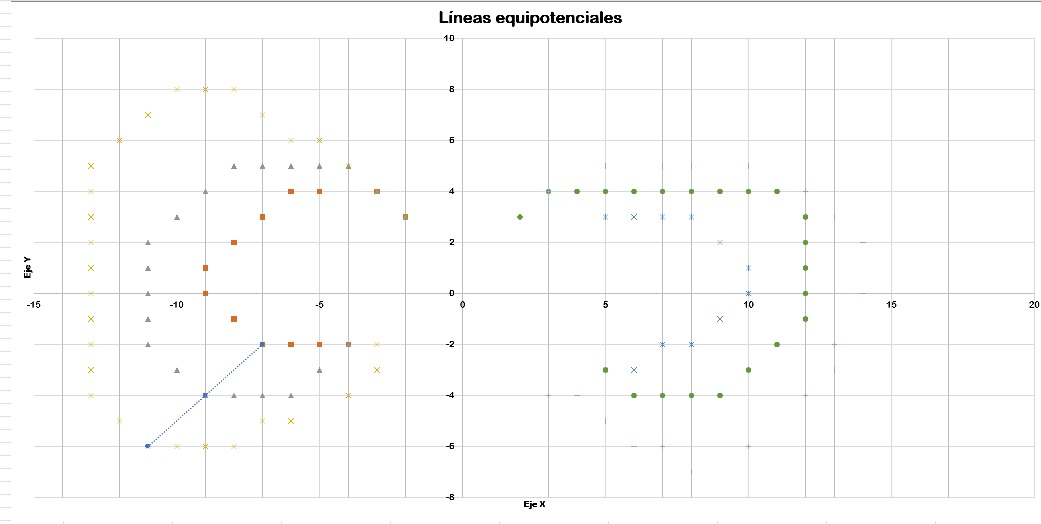
\includegraphics[scale=0.6]{imgs/g.jpeg}
	\caption{lineas equipotenciales}
	\label{Fig:1}
\end{figure}

Como se puede apreciar en la gráfica \ref{Fig:1}, se muestra una serie de puntos, estos puntos forman las llamadas líneas equipotenciales, que son las líneas que forman un campo eléctrico imaginario, en las cuales, si una partícula viaja a través de esa serie de puntos, su energía potencial sería la misma en cualquier punto del campo. La gráfica 1 muestra los 3 diferentes campos eléctricos medidos durante la sesión de laboratorio, en el cual cabe recalcar que, hacia la izquierda del eje Y, el nivel de voltaje iba disminuyendo conforme se avanzará en dirección del eje X, al igual que con el otro lado del eje, las cargas iban disminuyendo conforme se alejarán de la fuente de voltaje, esto debido a que la carga no llegaba con la misma intensidad a todas las distancias del plano.
\section{Conclusiones}\label{Conclusiones}				% -------------------- Conclusiones
Como nuestra principal conclusión, con ayuda de nuestros resultados obtenidos y con entusiasmo declaramos que el objetivo de las 3 prácticas se ha cumplido
y también es necesario contemplar las siguientes conclusiones, las temáticas de fuerza de carga, depósito de carga y líneas equipotenciales son fundamentales en el estudio de los campos eléctricos. 

La fuerza de carga es una medida de la interacción entre cargas eléctricas. Esta fuerza puede ser atractiva o repulsiva dependiendo del tipo de cargas involucradas. En los experimentos que realizaste, pudiste observar cómo diferentes materiales interactúan entre sí generando diferentes tipos de cargas.

El depósito de carga se refiere a cómo se distribuye la carga eléctrica en un sistema. En tu práctica, mediste la carga depositada en la jaula interna y externa de Faraday, observando cómo cambiaba esta distribución al interactuar con diferentes materiales y bajo diferentes condiciones.

Las líneas equipotenciales son una representación gráfica de los puntos en el espacio donde el potencial eléctrico es constante. Al dibujar estas líneas, pudiste visualizar la distribución general del campo eléctrico y entender cómo interactúan las cargas eléctricas dentro del sistema.

En conclusión, estos conceptos nos permiten entender mejor el comportamiento de los campos eléctricos y cómo las cargas interactúan entre sí. Cada material tiene propiedades únicas que afectan la forma en que interactúa con la carga eléctrica, lo que a su vez afecta la distribución del campo eléctrico en el sistema.

\begin{thebibliography}{9}						% -------------------- Bibliografía
	\bibitem{Martín}
		Martín, I. (2004). Física General
		\bibitem{Serway}
		Serway, R. A., $\&$ Jewett, J. W. (2008). Física para ciencias e ingeniería. (7.a
ed., Vol. 1). CENGAGE Learning.

\bibitem{Pérez}
	Newton, I. (1687). Philosophiæ Naturalis Principia Mathematica [Mathematical Principles of Natural Philosophy]. Londini: Jussu Societatis Regiæ ac Typis Josephi Streater.

\bibitem{Khan Academy}
	Anonymous. (2017). ¿Qué es la fricción? based on \cite{Openstax College Physics}. "from https://es.khanacademy.org/science/physics/forces-newtons-laws/inclined-planes-friction/a/what-is-friction"
	\bibitem{Openstax College Physics}
		Openstax College Physics. (n.d). Friction. from http://cnx.org/contents/031da8d3-b525-429c-80cf-6c8ed997733a@9,4:32/Friction"

\end{thebibliography}
\end{document}	